
\chapter{基于后缀树的重复记录检测}
\label{chap:suffixtree}

\section{后缀树简介}
\label{sec:suffixtreeintro}
后缀树(Suffix Tree)是一种可以快速高效实现许多字符串操作的数据结构。Weiner最早
在\cite{weiner1973linear}中提出了后缀树的概
念,Ukkonen在\cite{ukkonen1995line}中提出了一个$O(n)$时间复杂度的在线构造算
法。

后缀树实际上是前缀树(Trie树)的一种特殊形式。后缀树的每一条边都代表着一个序列,从
根节点到后缀树叶子节点的每条路径都对应着原序列的一个后缀。也就是说,后缀树其实就
是由序列所有后缀所组成的前缀树。举个例子,对于字符串{APPLE},其所有的后缀
为:\\
APPLE\\
PPLE\\
PLE\\
LE\\
E\\
对应的后缀树如\reffig{suffixtree:fig:suffix-tree-apple}所示。
从\reffig{suffixtree:fig:suffix-tree-apple}中可以看到,共有5条从根节点到叶子节点
的路径,每一条路径都对应于一条后缀。
\begin{figure}[h]
  \centering
  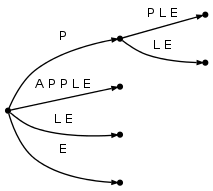
\includegraphics[width=0.4\textwidth]{suffixtree03/suffix-tree-apple}
  \caption{APPLE对应的后缀树}
  \label{suffixtree:fig:suffix-tree-apple}
\end{figure}

我们可以总结出序列$S$的后缀树有以下几个特点:
\begin{enumerate}
\item 所有的边都对应$S$的长度至少为1的非空的子序列
\item 从根到叶子节点的路径序列和序列S的后缀一一对应
\item 所有的内部节点(根节点不一定)都有至少两个子节点
\end{enumerate}

\section{Ukkonen后缀树构建算法}
\label{sec:ukkonen}
最简单的后缀树算法是先取出序列所有的后缀,然后按照前缀树的构造方法构造序列的后缀
树。这种方法虽然简单,但是复杂度较高,不适用于数据量较大的情况。为了高效地实现重
复记录检测的模块,我们的系统实现了Ukkonen在\cite{ukkonen1995line}中提出的时
间复杂度为$O(n)$的后缀树在线构建算法。以下将以字符串{BANANA}为例,简单介绍
这种在线算法的构造过程。由于这个算法比较复杂,以下的这个例子并不能涵盖算法的所有
细节。

首先我们引入3个状态变量描述某一个时刻对应的后缀树的构造状态。

第一个状态变量是{\#},表示序列中扫描到的最后一个元素的位置。初始值为0,表
示第一个元素,在以后的每轮迭代中,\#的值将加1,当\#的值和序列的长度相同时迭代终
止。
  
第二个是{activePoint},用于表示下一次要在后缀树插入新的点时的位置,为了确
定这样一个唯一的位置,我们需要一个三元组{(activeNode, activeEdge,
  activeLength)}表示{activePoint},这三个变量分别表示当前后缀树的某个节点,
该节点的某条边以及这条边上第几个元素。初始值为{(root, '', 0)},表示初始的
插入操作都在根节点{root}上进行。下面
以\reffig{suffixtree:fig:suffix-tree-apple}中的后缀树为例简要说明:若
用{root}表示根节点,则当{activePoint}为{(root, A, 3)}时意味
着下一次插入新的点的位置应该是从根节点{root}的以字母{A}开头的边的
第3个字符后面,即{root}的{APPLE}对应的边的第二个{P}字母后面
的位置。
  
第三个状态变量是{remainder},表示当前还需要往后缀树中插入几次后缀。初始值
为1。

对于我们的输入{BANANA}来说,最后一个字母是{A},这个字母在字符串之前
的某个位置中出现过({BANANA}共有3个字母{A}),因此需要在输入串的末
尾增加一个终结符,以保证输入的最后一个字符没有在之前出现过,我们这里采用\$。因此,
原始的输入{BANANA}就变成了{BANANA\$}

一开始的时候,我们只有一个根节点,\#为0,插入后缀{B},变
成\reffig{suffixtree:fig:1}所示的图;下一轮迭代\#值增加到1,新的后缀{A}在
原来的边中没有出现,插入一条新的边,得到\reffig{suffixtree:fig:2};接下来\#增加
到2,和前一步一样,新的后缀{N}没有在原来的边中出现过,插入一条新的边,得
到\reffig{suffixtree:fig:3}。目前为止,{activePoint}和{remainder}都
没发生变化。

接下来\#加1,将导致需要插入一条新的后缀{A},但是我们发现{A}已经在之
前的边中出现过,因此这时我们不插入新的边,而将{activePoint}更新
为{(root,A,1)},{remainder}加1,此时后缀树
如\reffig{suffixtree:fig:4}所示,边数没有发生变化,但是状态变量发生了改变。下一
步\#再加1,由于此时{remainder}为2,因此我们需要将新的后缀{N}往后缀
树中插入两次。从{activePoint}出发,我们发现下一个字母正好是{N},因
此我们不再试图往后缀树中插入{N}了,而是
将{activePoint}和{remainder}分别更新为{(root,A,2)}和3。下一
轮迭代也是类似,在插入最后一个\$之前,后缀树如\reffig{suffixtree:fig:6}所示,
{activePoint}和{remainder}的值分别为{(root, A, 3)}和4。
% 插入后缀树构造的图片

\begin{figure}
  \begin{subfigure}[t]{0.33\linewidth}
    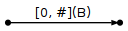
\includegraphics[width=0.8\textwidth]{suffixtree03/suffixtree-1}
    \caption{\#=0}
    \label{suffixtree:fig:1}
  \end{subfigure}
  \begin{subfigure}[t]{0.33\linewidth}
    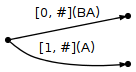
\includegraphics[width=0.8\textwidth]{suffixtree03/suffixtree-2}
        \caption{\#=1}
    \label{suffixtree:fig:2}
  \end{subfigure}
    \begin{subfigure}[t]{0.33\linewidth}
    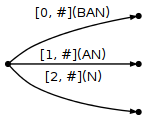
\includegraphics[width=0.8\textwidth]{suffixtree03/suffixtree-3}
        \caption{\#=2}
    \label{suffixtree:fig:3}
  \end{subfigure}
  \begin{subfigure}[t]{0.33\linewidth}
    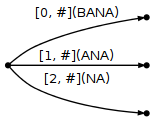
\includegraphics[width=0.8\textwidth]{suffixtree03/suffixtree-4}
    \caption{\#=3}
    \label{suffixtree:fig:4}
  \end{subfigure}
  \begin{subfigure}[t]{0.33\linewidth}
    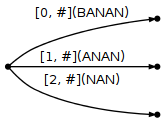
\includegraphics[width=0.8\textwidth]{suffixtree03/suffixtree-5}
        \caption{\#=4}
    \label{suffixtree:fig:5}
  \end{subfigure}
    \begin{subfigure}[t]{0.33\linewidth}
    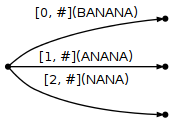
\includegraphics[width=0.8\textwidth]{suffixtree03/suffixtree-6}
        \caption{\#=5}
    \label{suffixtree:fig:6}
  \end{subfigure}
  \caption{前六轮迭代(\#从0到5)中的后缀树变化}
  \label{suffixtree:fig:0to5}
\end{figure}
\begin{figure}
  \begin{subfigure}[t]{0.5\linewidth}
    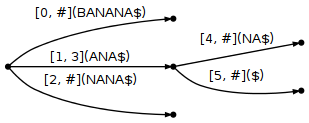
\includegraphics[width=\textwidth]{suffixtree03/suffixtree-7-1}
    \caption{remainder=4}
    \label{suffixtree:fig:7-1}
  \end{subfigure}
  \begin{subfigure}[t]{0.5\linewidth}
    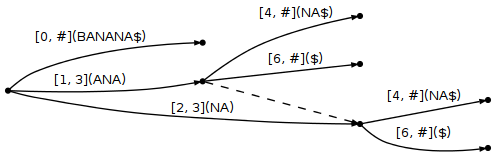
\includegraphics[width=\textwidth]{suffixtree03/suffixtree-7-2}
        \caption{remainder=3}
    \label{suffixtree:fig:7-2}
  \end{subfigure}
  \begin{subfigure}[t]{0.5\textwidth}
    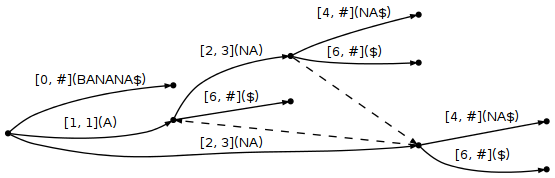
\includegraphics[width=\textwidth]{suffixtree03/suffixtree-7-3}
    \caption{remainder=2}
    \label{suffixtree:fig:7-3}
  \end{subfigure}
  \begin{subfigure}[t]{0.5\textwidth}
    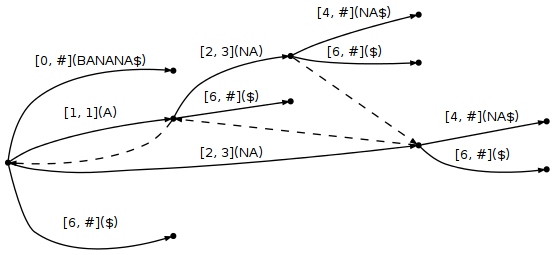
\includegraphics[width=\textwidth]{suffixtree03/suffixtree-7-4}
    \caption{remainder=1}
    \label{suffixtree:fig:7-4}
\end{subfigure}
\caption{最后一轮迭代(\#=6)时的后缀树}
\label{suffixtree:fig:7}
\end{figure}

%%% Local Variables: 
%%% mode: latex
%%% TeX-master: "../main"
%%% End: 


最后一轮迭代,我们需要插入终止符\$。从此时的{activePoint}出发,发现下一个
字母和和\$并不匹配,此时我们需要往后缀树中插入\$字符,方法是
在{activePoint}对应的位置生成一个新的内部节点,并在新生成的节点的地方插入
一条边,表示\$,如\reffig{suffixtree:fig:7}所示。我们需要更
新{activePoint}的值:将{activeNode}移到根节点处(在这个例子中实际上
没有移动),对应的边是以原来的{activeEdge}的第2个字母开头的边,
即{N},{activeLength}减1。{remainder}的值也减1,变为3,也就
是我们还需要插入3次\$。接下来的两次插入和我们第一次插入时的情况一样,会新生成两个
内部节点;最后一次插入则和一开始的情况一样,我们直接在根节点处插入\$。最后一轮迭
代的过程如\reffig{suffixtree:fig:7}所示,最后生成的完整的后缀树
如\reffig{suffixtree:fig:7-4}所示。

在最后的\reffig{suffixtree:fig:7-4}中,我们看到还有一些连接几个内部节点之间的有向
的虚线,我们之前没有提到,这是后缀链(Suffix Link)。我们例子中的后缀链都是在最后
一轮迭代插入\$时生成的。关于后缀链生成的简单的规则是:在同一轮迭代中,如果在某一
步中某个节点处发生了一次插入,则要从这一轮迭代之前生成内部节点(如果有的话)引一
条后缀链指向该节点。后缀链的作用是如果在某个带有后缀链的节点发生了插入,则在更
新{activePoint}时把其中的{activeNode}更新为沿着后缀链连接的那个节点,
而不是根节点。后缀链不影响前述的其他规则。限于篇幅,我们不再具体举例说明后缀链的
使用方法。

\section{重复记录检测算法}
\label{sec:multipldetect}

\subsection{后缀树检测重复序列的基本算法}
依照~\ref{sec:ukkonen}所述的后缀树构造算法,我们给每一个DOM Tree的先序遍历序列构
造一个后缀树,然后根据后缀树检测其中重复的记录。

根据后缀树构造的特点,任意一条从根节点到内部节点的路径组成的序列都是原序列中重复
出现的子序列,且重复的次数是以该内部节点为根的子树的叶子节点个数。
在\reffig{suffixtree:fig:7-4}中,{A},{ANA},{NA}都是
{BANANA}的重复子串,分别重复出现了3次,2次和2次。这种方法有以下几个问题:
\begin{itemize}
\item 不同的重复子串之间可能有包含或者相交的关系。在之前的例子中,{ANA}包
  含了{NA}和{A}。
\item 同一个重复子串在原序列上有交集。比如{ANA},对应到原序列上的两个子序
  列有交集{A}。  
\end{itemize}

直接采用上面的方法查找后缀树中的重复记录是不可行的。我们从DOM Tree得到先序遍历序
列和普通的序列不一样,里面是包含有原始的树的结构信息的。我们需要检测的重复记录必
须位于同一个子树上,有公共的父亲。这个特点对应到序列上,必须要求:
\begin{itemize}
\item 重复序列不能横跨两个子树
\item 重复序列必须有公共的父亲
\end{itemize}

此外,我们还要求这个重复序列必须尽可能地长。

\subsection{改进的检测算法}
因此,我们需要进一步对原来的重复序列查找算法进行改进。算
法~\ref{suffixtree:algo:fromroot}和\ref{suffixtree:algo:findrep}给出了我们查找所
有符合我们要求的重复子序列的算法。

% 输入代码文件
\begin{algorithm}
  \caption{从根节点出发,找出所有的重复子序列\label{suffixtree:algo:fromroot}}
  \begin{algorithmic}[1]
    \Require 已经构建好的后缀树,根为$root$
    \Ensure 该后缀树中所有的重复子序列
    \State $//$从节点出发,寻找所有的重复子序列
    \For{$edge \gets root.edges~\mathbf{if}~edge.endNode.isNotLeaf$}
    \State $//$取后缀树根节点的每条边的第一个元素作为每个子树的根节点
    \State $subTreeRoot := edge.firstElement$
    \State $//$查找以该节点为根的所有重复子序列
    \State findAllRepetitions$(root, \mathbf{nil}, subTreeRoot)$
    \EndFor
  \end{algorithmic}
\end{algorithm}

\begin{algorithm}
  \caption{找出后缀树中经过某个内部节点的所有可能的重复子序列}
  \label{suffixtree:algo:findrep}
  \begin{algorithmic}[1]
    \Require 一个内部节点$node$,当前已经找到的重复序列$prefix$,要找的
    子树的根节点$subTreeRoot$
    \Ensure 所有经过该内部节点的符合要求的重复序列
    \Function {findAllRepetitions}{$node, prefix, subTreeRoot$}
    \State $//$定义一个空集合
    \State $results := Collection.empty$
    \State $//$对于该内部节点的每一条不连接叶子节点的边
    \For{$edge \gets node.edges~\mathbf{if}~edge.endNode.isNotLeaf$}
    \State $//$依次取出该条边上元素的根节点可能为root的点
    \State $seq := edge.takeWhile(element$ inSubTreeOf $subTreeRoot)$\label{suffixtree:code:equals}
    \If {$seq.length == edge.length$}
    \State $//$遍历完了该条边上所有元素,
    \State $//$则取该条边连接的下一个内部节点进行递归查找
    \State findAllRepetitions($edge.endNode, prefix + seq, subTreeRoot$)
    \Else
    \State $//$否则,将当前得到的序列加入到结果集合中
    \State addToResults$(prefix + seq, results)$\label{suffixtree:code:add}
    \EndIf
    \EndFor
    \State \Return{$results$}
    \EndFunction
    \State
  \end{algorithmic}
\end{algorithm}

%%% Local Variables: 
%%% mode: latex
%%% TeX-master: "../main"
%%% End: 


根据算法~\ref{suffixtree:algo:fromroot}和~\ref{suffixtree:algo:findrep}得到的重复
子序列,可以保证不会横跨两个子树,且尽可能地长,但还有几点需要说明。

第一,根据算法~\ref{suffixtree:algo:fromroot}和~\ref{suffixtree:algo:findrep}得到
的在原序列中重复出现的子树的序列,不一定有相同的父亲节点,因此不能直接根据这个结
果去掉重复记录,还需要做进一步的处理。

第二,算法~\ref{suffixtree:algo:findrep}中的代码addToResults$(prefix + seq,
results)$将新的序列加入到结果集合中。实际在加入的时候,我们需要先将新的序列和结果
集合中已有的序列进行对比。如果结果集合中的某个序列被新的序列所包含,则我们用新的
序列代替原有的序列。这个操作可以在$O(1)$的时间内完成。因为在后缀树中,如果两个子
序列有包含关系,即$S_1$包含$S_2$,必然有$S_2$为$S_1$的后缀,这可以通过比
较$S_1$和$S_2$最后一个元素的下标是否相等来判断。

\subsection{合并重复记录}
接下来我们将对找出来的所有可能的重复序列进行合并。根据先序遍历的特点,子树的根节
点总是出现在该子树对应的序列的起始处。因此,对于我们找到的每一个重复的子序列,我
们总是可以通过向前搜索找到其父节点。接下来把所有的序列按照其父亲节点进行分类,然
后遍历每一个父节点所对应的全部重复序列$S_1,S_2,...,S_n$,若存在一个序列集
合${S_{i_1},S_{i_2},...,S_{i_k}}, i_1<i_2<...<i_k, k>1$,其中的每个序列都相等,则
只保留$S_{i_1}$,将其余全部去除。最后我们将在保留下来的$S_{i_1}$中设定标志位,表
明该序列在模板中是可以多次出现的。

我们实际的合并算法要比上述的稍复杂一些,因为有很多边界情况需要特殊处理。比如,算
法~\ref{suffixtree:algo:fromroot}和\ref{suffixtree:algo:findrep}虽然去除了序列横
跨两个子树和序列互相包含的问题,但是对于序列相交的情况,并没有做相应的处理。对于
以下的某个HTML标签序列片段(每个标签由{标签名+深度}组成):
\begin{center}
  ...<div3><div4><div3><div4><a5><img5><div4><a5><img5>...
\end{center}
按照之前的算法,我们可以找到的符合条件的重复序列包
括{<div3><div4>}和{<div4><a5><img5>}。但是这两个序列实际上有交
集:{<div4>}。我们采取的策略是只取更深的重复序列。在这个例子中,我们保
留{<div4><a5><img5>},将第二个{<div3><div4>}序列从重复序列集合中去
掉。

实际处理中其他还有一些类似的边界条件,这里就不再赘述了。

\section{本章小结}
\label{sec:summarysuffixtree}
本章主要对预处理模块中的重复记录检测子模块进行了详细描述。先简单介绍了后缀树的定
义和性质,然后举了一个具体的例子说明如何在$O(n)$时间内在线构建出一个序列的后缀树,
最后对利用后缀树进行重复记录检测的算法做了详细的介绍和说明。

这个子模块是预处理模块中最重要的一个。如果我们不对网页中重复的记录进行处理,这些
不定个数的重复记录将成为后续的聚类和模板提取过程中很大的噪音,大大减小聚类和模板
提取的精度。由于我们实现并使用了后缀树这种高效的数据结构,使得我们的算法可以很快
找出所有符合条件的重复序列,并将它们正确地进行合并。

%%% Local Variables: 
%%% mode: latex
%%% TeX-master: "../main"
%%% End: 
